\section{Installation}
\subsection{Setting Up the Wazuh Server}

There are two methods to setup the Wazuh Server:

\subsubsection{Quickstart Installation}
We adopted this way to install the Wazuh Server. This is a straightforward all-in-one installation and is suitable for small-scale deployments. The following steps are involved in the installation process:
\begin{enumerate}
  \item Download and run the Wazuh installation assistant.

  \begin{minted}[tabsize=2,breaklines=true,breakanywhere=true,bgcolor=LightGray]{bash}
curl -sO https://packages.wazuh.com/4.7/wazuh-install.sh && sudo bash ./wazuh-install.sh -a
  \end{minted}

  \item Once the assistant finishes, the output will display the access credentials and confirm successful installation.

  \begin{minted}[tabsize=2,breaklines=true,breakanywhere=true,bgcolor=LightGray]{text}
INFO: --- Summary ---
INFO: You can access the web interface https://<wazuh-dashboard-ip>
User: admin
Password: <ADMIN_PASSWORD>
INFO: Installation finished.
  \end{minted}

  Make sure to save the credentials for future usage. It will be used to access the dashboard.

  \item Access the Wazuh web interface at \url{https://<wazuh-dashboard-ip>} using the provided credentials:

    \begin{minted}[tabsize=2,breaklines=true,breakanywhere=true,bgcolor=LightGray]{text}
Username: admin
Password: <ADMIN_PASSWORD>
    \end{minted}

  \item Upon first access, a browser warning about the certificate may appear. This is normal because the certificate was not issued by a recognized authority. You may accept the certificate as an exception or configure a certificate from a trusted authority.

  \item The passwords for all Wazuh indexer and Wazuh API users can be found in the file named \texttt{wazuh-passwords.txt}, which is inside \texttt{wazuh-install-files.tar}. To display them, execute:
  \begin{minted}[tabsize=2,breaklines=true,breakanywhere=true,bgcolor=LightGray]{bash}
sudo tar -O -xvf wazuh-install-files.tar && wazuh-install-files/wazuh-passwords.txt
  \end{minted}

  \item To uninstall Wazuh's central components, execute the installation assistant with the option \texttt{-u} or \texttt{--uninstall}.
\end{enumerate}

\subsubsection{Step-by-step Installation of the Wazuh Indexer, Manager and Dashboard}

Please refer to the Wazuh official documentation \href{https://documentation.wazuh.com/current/installation-guide/wazuh-dashboard/step-by-step.html}{page} for the step-by-step installation of the Wazuh Server components. This provides more in-depth insight and fine-grained control over different details of the installation process.

\subsection{Registering Agents}
Registering new agents becomes way too easy once the server is set up. The procedure is stated as follows:
\begin{itemize}
  \item Go to Agents \(\rightarrow\) Deploy New Agent as shown in the following image:
    \begin{figure}[H]
      \centering
      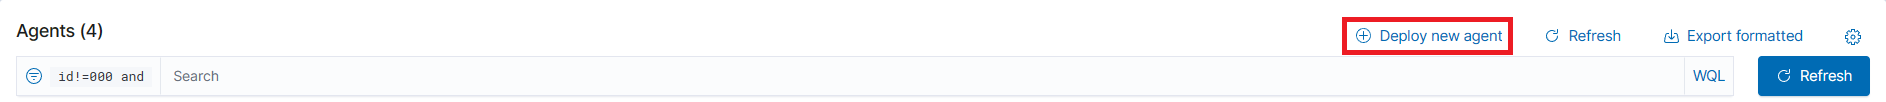
\includegraphics[width=\textwidth]{images/newagent-option.png}
      \caption{Wazuh Dashboard - Deploy New Agent}
    \end{figure}
  \item There, provide the necessary information like Agent OS, Server address, Agent name and Agent group (last two are optional).
  \item Finally, two sets of commands will be shown, running which should be enough to install and initiate Wazuh Agent on the given machine.
  \begin{itemize}
    \item \textbf{Linux:}
    \begin{figure}[H]
      \centering
      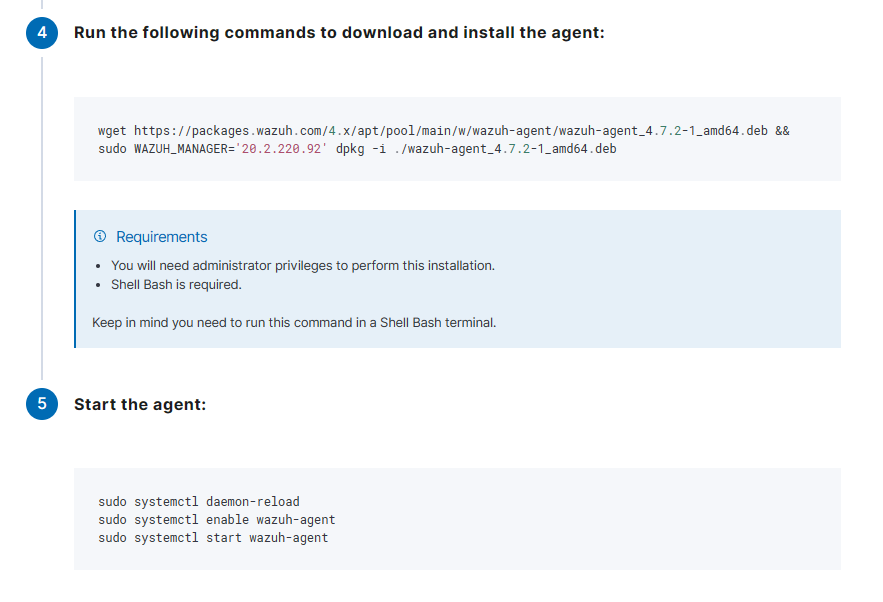
\includegraphics[width=0.6\textwidth]{images/wazuh-agent-commands-linux.png}
      \caption{Wazuh Agent Installation Commands for a Linux Machine}
    \end{figure}
    \begin{minted}[tabsize=2,breaklines=true,breakanywhere=true,bgcolor=LightGray]{bash}
wget https://packages.wazuh.com/4.x/apt/pool/main/w/wazuh-agent/wazuh-agent_4.7.2-1_amd64.deb && sudo WAZUH_MANAGER='20.2.220.92' dpkg -i ./wazuh-agent_4.7.2-1_amd64.deb
sudo systemctl daemon-reload
sudo systemctl enable wazuh-agent
sudo systemctl start wazuh-agent
    \end{minted}

    \item \textbf{MacOS:}
    \begin{figure}[H]
      \centering
      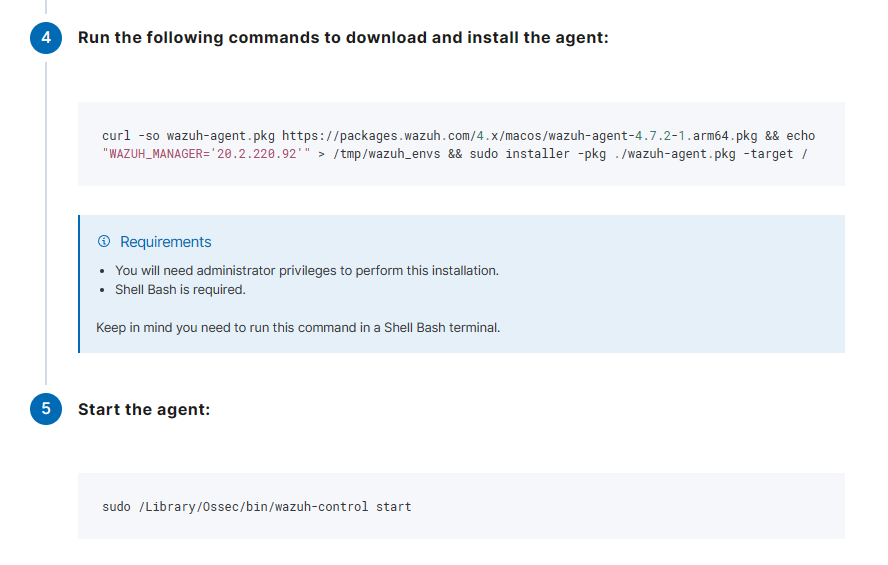
\includegraphics[width=0.6\textwidth]{images/wazuh-agent-commands-mac.png}
      \caption{Wazuh Agent Installation Commands for a macOS Machine}
    \end{figure}
    \begin{minted}[tabsize=2,breaklines=true,breakanywhere=true,bgcolor=LightGray]{bash}
curl -so wazuh-agent.pkg https://packages.wazuh.com/4.x/macos/wazuh-agent-4.7.2-1.arm64.pkg && echo "WAZUH_MANAGER='20.2.220.92'" > /tmp/wazuh_envs && sudo installer -pkg ./wazuh-agent.pkg -target /
sudo /Library/Ossec/bin/wazuh-control start
    \end{minted}

    \item \textbf{Windows:}
    \begin{figure}[H]
      \centering
      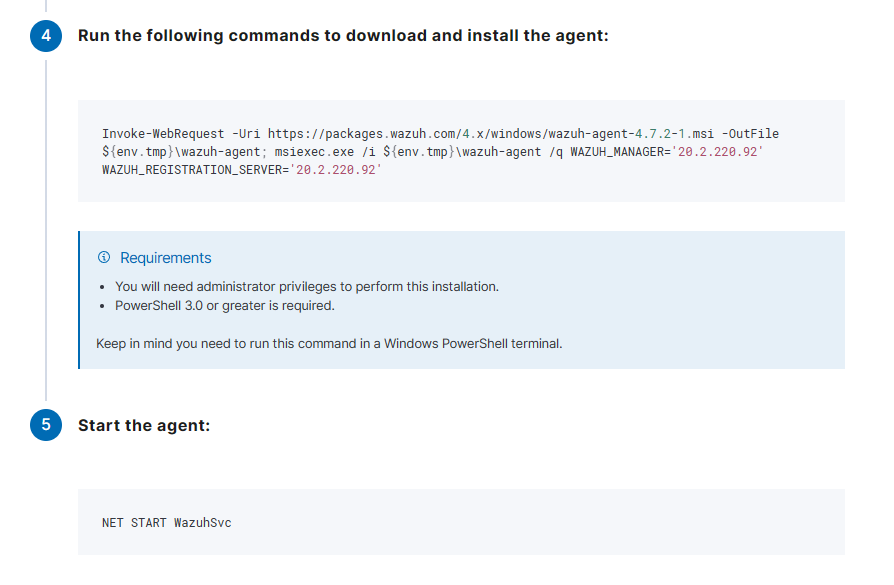
\includegraphics[width=0.6\textwidth]{images/wazuh-agent-commands-win.png}
      \caption{Wazuh Agent Installation Commands for a Windows}
    \end{figure}
    \begin{minted}[tabsize=2,breaklines=true,breakanywhere=true,bgcolor=LightGray]{bash}
Invoke-WebRequest -Uri https://packages.wazuh.com/4.x/windows/wazuh-agent-4.7.2-1.msi -OutFile ${env.tmp}\wazuh-agent; msiexec.exe /i ${env.tmp}\wazuh-agent /q WAZUH_MANAGER='20.2.220.92' WAZUH_REGISTRATION_SERVER='20.2.220.92' 
NET START WazuhSvc
    \end{minted}
\end{itemize}

  \end{itemize}
